\section{Low Power Mode}
\label{sec:LOWPOWERMODE}

A typical SoC has a low power controller to put the CPU core into low power mode. It seems that your SoC with mmRISC-1 has a similar configuration as shown in Figure \ref{fig:LOWPOWERBLOCKDIAGRAM}.\\

The control timing is described below. As shown in Figure \ref{fig:LOWPOWERTIMING}, please assert STBY\_REQ when the low power controller recieves a STBY request to put the CPU into low power consumption mode. All HARTs in mmRISC-1 temporarily stop executing instructions, and each HART asserts the stby\_ack signal once all instruction executions in the pipeline become empty. After all HART's stby\_acks are asserted, mmRISC-1 asserts the STBY\_ACK signal to inform the low power controller that mmRISC-1 has entered to STBY state.\\
After that, the low power controller should stop the system clock to the CPU. Then, the mmRISC-1 becomes physically low power consumption state. The reason why the CPU flushes the pipeline before entering a low power state is to prevent the clock from stopping while the instruction or data memory access is incomplete.\\

To exit from the low power consumption state, please restart the clock to the CPU before negating the STBY\_REQ signal. The mmRISC-1 negates the STBY\_ACK signal and each hart resumes instruction execution.\\

\begin{figure}[H]
    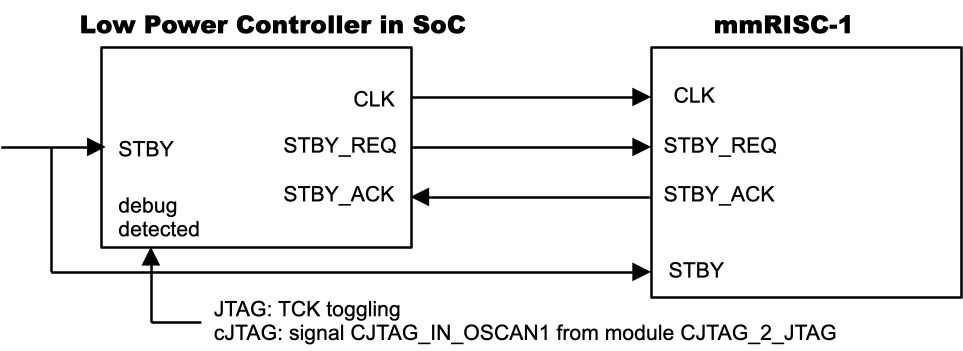
\includegraphics[width=1.00\columnwidth]{./Figure/LowPowerBlockDiagram.png}
    \caption{Block Diagram of Low Power Support}
    \label{fig:LOWPOWERBLOCKDIAGRAM}
\end{figure}

\begin{figure}[H]
    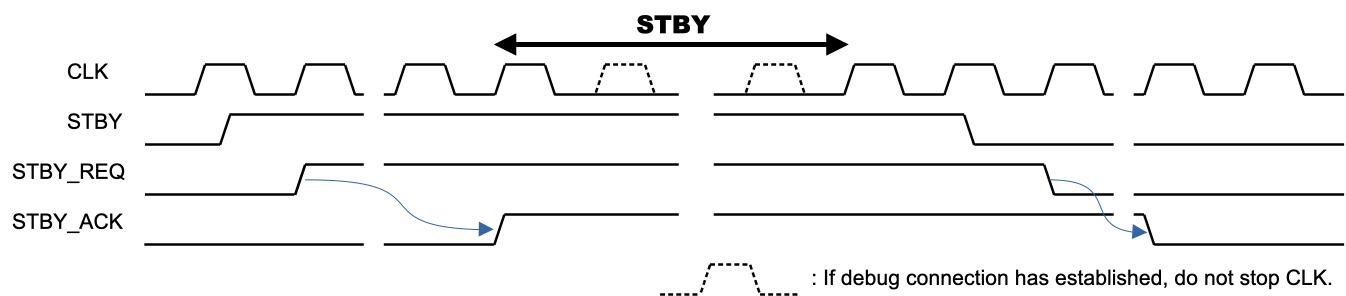
\includegraphics[width=1.00\columnwidth]{./Figure/LowPowerTiming.png}
    \caption{Timing of Low Power Support}
    \label{fig:LOWPOWERTIMING}
\end{figure}

\it{Note 1 : An output signal STBY\_ACK shows that mmRISC-1 core enters low power mode. During the state, if the system clock is stopping, when a debugger such as OpenOCD accesses the mmRISC-1 via JTAG or cJTAG interface, the access will fail because JTAG DTM (Debug Transport Module) requires toggling CLK (System Clock). So, once a debug transaction on JTAG/cJTAG occurs, the low power controller should not stop CLK even when a low power transaction described above. The way to detect the debug transaction is (1) For, 4-wire JTAG, Detecting TCK Toggling, or (2) For 2-wire cJTAG, Detecting CJTAG\_IN\_OSCAN1 is high level.}\rm\\

\it{Note 2 : Even when in STBY state, the debugger can access mmRISC-1 if CLK does not stop. But if the Hart-Available status implemented in DMSTATUS register of DM (Debug Module) shows "Unavailable" during STBY, the debugger might report access errors. You can select whether the Hart-Available status in DMSTATUS is reflected by STBY state or not by setting UNAVAILABLE\_WHEN\_STBY switch in defines\_core.v. The default setting is that the switch is OFF and Hart-Available status is always 1.}\rm{}


